%  V E R Z E I C H N I S S E


\clearpage{\pagestyle{empty}\cleardoublepage}

\addtocontents{toc}{\vspace{5mm}}
\addpart[\large\uppercase{Verzeichnisse}]{\protect\textso{VERZEICHNISSE}}
\clearpage{\pagestyle{empty}\cleardoublepage}
\renewcommand*{\chapterpagestyle}{empty}
 	
 				    			    
% PERSONENVERZEICHNIS
\small
\setindexpreamble{\vskip4ex%
Kaiser werden unter dem Stichwort Kaiser mit nachfolgendem Namen, 
P\"{a}pste unter dem Stichwort Papst mit nachfolgendem Namen aufgef\"{u}hrt. 
Andere Regenten werden unter dem Namen des von ihnen regierten Staates gelistet. 
Bei diesen Personengruppen sind die Jahreszahlen Regierungszeiten, bei allen anderen Lebensdaten. 
Bei Autoren ist zus\"{a}tzlich das Schriftenverzeichnis heranzuziehen. 
Es wird nach Seiten zitiert. Kursive Seitenzahlen verweisen auf den Apparat-Teil.\vskip4ex}
\addcontentsline{toc}{chapter}{\enskip Personen}
\markleft{\scriptsize\uppercase{Verzeichnisse}}
\printindex{Namensregister}{PERSONEN}


% SCRIFTENVERZEICHNIS
\clearscrheadfoot
\chead{\sc{Schriften}}
\ohead[\pagemark]{\pagemark}
\begin{multicols}{2}[\footnotesize\addchap*{\hfill SCHRIFTEN\hfill}
\addcontentsline{toc}{chapter}{\enskip Schriften}
\vspace{15pt}
Das Schriftenverzeichnis enth\"{a}lt die Literatur der Leibnizzeit und die in den Erl\"{a}uterungen 
benutzte Literatur. Es wird nach Seiten zitiert. Kursive Seitenzahlen verweisen auf den Apparat-Teil.\\]
\setlength{\columnseprule}{0.4pt}					
\renewcommand*{\chapter}{\OrigChapter}
\bibliographystyle{leibniz8bib}
\footnotesize
\bibliography{l8bib}{}
\end{multicols}    


% SACHVERZEICHNIS
\setindexpreamble{\vskip4ex%
Eintr\"{a}ge in dieses Verzeichnis erfolgen in der jeweils von Leibniz verwendeten Sprache. 
Die Reihenfolge der Eintr\"{a}ge ist rein alphabetisch bestimmt, 
eine systematische Gliederung findet nicht statt. 
Es wird nach Seiten zitiert. Kursive Seitenzahlen verweisen auf den Apparat-Teil. \vskip4ex}
\addcontentsline{toc}{chapter}{\enskip Sachen}
\printindex{Sachverzeichnis}{SACHEN} 


% ORTSVERZEICHNIS
\setindexpreamble{\vskip4ex%
Dieses Verzeichnis listet alle von Leibniz genannten Ortsnamen in ihrer deutschen Version auf. 
Es wird nach Seiten zitiert. Kursive Seitenzahlen verweisen auf den Apparat-Teil.\vskip4ex}
\addcontentsline{toc}{chapter}{\enskip Orte}
\printindex{Ortsregister}{ORTE}  
       

% FUNDSTELLENVERZEICHNIS
\clearscrheadfoot
\chead{\sc{Fundstellen}}
\ohead[\pagemark]{\pagemark}
\clearpage{\pagestyle{empty}\cleardoublepage}
\setindexpreamble{\vskip4ex%
% ???? 
\vskip4ex}
\addcontentsline{toc}{chapter}{\enskip Fundstellen}
    \thispagestyle{empty}
\vspace{3.0ex}
\begin{center}\uppercase{\normalsize Fundstellen}\end{center}
\footnotesize
Folgendes Register verzeichnet sämtliche im vorliegenden Band edierten Hand- und Druckschriften, 
alpha\-betisch geordnet nach \mbox{Fund\-ort} und Signatur.\\[4.0ex]%
%%
\textsc{Druckschrift}\\
\vspace{-3mm}
\setlength{\columnseprule}{0.4pt}
\renewcommand*{\chapter}{\OrigChapter}
\setlength\LTleft{\fill} \setlength\LTright{\fill}
\begin{longtable}{ll}
\footnotesize
\textit{Journal général de l'Instruction publique et des cultes} XXVI (1857), Nr. 32, S. 235f. & N. 81\\%% = ex N. 93 = RK ?????.
\end{longtable}
\vspace{3.0ex}
%%
\noindent
\textsc{Göttingen}, \textit{Niedersächsische Staats- und Universitätsbibliothek}\\ 
\vspace{-3mm}
\setlength{\columnseprule}{0.4pt}
\renewcommand*{\chapter}{\OrigChapter}
\setlength\LTleft{\fill} \setlength\LTright{\fill}
\begin{longtable}{ll}
\footnotesize
8 MED PRACT 96/37 & N. 67\\%% = ex N. 84 = RK 62029.
\end{longtable}
\vspace{3.0ex}
%%
\noindent
\textsc{Göttingen}, \textit{Stadtarchiv}\\ 
\vspace{-3mm}
\setlength{\columnseprule}{0.4pt}
\renewcommand*{\chapter}{\OrigChapter}
\setlength\LTleft{\fill} \setlength\LTright{\fill}
\begin{longtable}{ll}
\footnotesize
MSL Nr. 12 Bl. 19 & N. 66\\%% = ex N. 74 = RK 60389.
\end{longtable}
\vspace{3.0ex}
%%
\noindent
\textsc{Hannover}, \textit{Gottfried Wilhelm Leibniz Bibliothek \textendash\ Niedersächsische Landesbibliothek}\\
\vspace{-3mm}
\setlength{\columnseprule}{0.4pt}
\renewcommand*{\chapter}{\OrigChapter}
\setlength\LTleft{\fill} \setlength\LTright{\fill}
\begin{longtable}{llll}
\footnotesize
LBr & 719a          & Bl. 3\textendash 4 & N. 57\\%% = ex N. 64 = Cc2 00 = RK 41946.
LH III & 1, 3 & Bl. 1\textendash 8 & N. 70\\%% = ex N. 75 = KK1 975.
LH III & 1, 3 & Bl. 9 & N. 69\\%% = ex N. 76 = KK1 976.
% LH III & 3, 3a & Bl. 11\textendash 12 & N. ***\\%%    N. *77 = Cc2 1562.
% LH III & 3, 3a & Bl. 19\textendash 22 & N. ***\\%%    N. *78 = KK1 978.
LH III & 4, 3a & Bl. 1 & N. 76\\%% = ex  N. 79 = Cc2 1323 A (tlw.).
LH III & 4, 3a & Bl. 1 & N. 82\\%% = ex N. 96 = Cc2 1323 A (tlw.).
LH III & 4, 8a & Bl. 1 & N. 74\\%% = ex N. 80 = Cc2 1563.
LH III & 5 & Bl. 49 & N. 76\\%% = ex N. 79 = Cc2 1323 B.
LH III & 5 & Bl. 55 & N. 71\\%% = ex N. 81 = KK1 977.
LH III & 5 & Bl. 56 & N. 75\\%% = ex N. 82 = Cc2 1271.
LH III & 5 & Bl. 67\textendash 68 & N. 68\\%% = ex N. 83 = KK1 979.
LH III & 5 & Bl. 86\textendash 87 & N. 73\\%% = ex N. 85 = Cc2 430.
% LH III & 5 & Bl. 88 & N. ***\\%%    N. *86 = Cc2 340.
LH III & 5 & Bl. 89 & N. 72\\%% = ex N. 87 = Cc2 869.
LH IV & 1, 4b & Bl. 3\textendash 12 & N. 58\\%% = ex N. 68 = Cc2 1322 A-E (D tlw.).
LH IV & 1, 4b & Bl. 9\textendash 10 & N. 6\\%% = ex N. 62 = Cc2 1322 D (tlw.) = RK 60606.
LH IV & 1, 4b & Bl. 13\textendash 14 & N. 54\\%% = ex N. 68 = Cc2 1324.
LH XXXV & 2, 1 & Bl. 273 & N. 95\\%% = ex N. 06 = Cc2 897 (tlw.).
LH XXXV & 5, 23 & Bl. 14 & N. 96\\%% = ex N. 95 = Cc2 00 = RK 58394.??
LH XXXV & 8, 30 & Bl. 151 & N. 11\\%% = ex N. 54 = Cc2 939.
LH XXXV & 9, 11 & Bl. 1\textendash 2 & N. 36\textsubscript{1}\\%% = ex N. 31/1 = Cc2 1189 A, C.
LH XXXV & 9, 11 & Bl. 3\textendash 4 & N. 36\textsubscript{2}\\%% = ex N. 31/2 = Cc2 1189 B, D-G.
LH XXXV & 9, 11 & Bl. 5\textendash 8 & N. 34\textsubscript{1}\\%% = ex N. 29/1 = Cc2 965 A-C, G-H.
LH XXXV & 9, 11 & Bl. 7\textendash 10 & N. 34\textsubscript{2}\\%% = ex N. 29/2 = Cc2 965 D, K.
LH XXXV & 9, 11 & Bl. 9\textendash 12 & N. 34\textsubscript{3}\\%% = ex N. 29/3 = Cc2 965 E, J.
LH XXXV & 9, 11 & Bl. 11\textendash 14 & N. 34\textsubscript{4}\\%% = ex N. 29/4 = Cc2 965 F.
LH XXXV & 9, 11 & Bl. 13\textendash 14 & N. 34\textsubscript{5}\\%% = ex N. 29/5 = Cc2 00 = (RK 41140).
LH XXXV & 10, 9 & Bl. 1 & N. 28\textsubscript{4}\\%% = ex N. 22/4 = Cc2 1190 A.
LH XXXV & 10, 9 & Bl. 2 & N. 28\textsubscript{3}\\%% = ex N. 22/3 = Cc2 1190 B.
LH XXXV & 10, 9 & Bl. 3\textendash 4 & N. 5\\%% = ex N. 61 = Cc2 1191 (tlw.) (3r).
LH XXXV & 10, 9 & Bl. 3\textendash 4 & N. 28\textsubscript{1}\\%% = ex N. 22/1 = Cc2 1190 D (3v).
LH XXXV & 10, 9 & Bl. 3\textendash 4 & N. 28\textsubscript{2}\\%% = ex N. 22/2 = Cc2 1190 C (3v).
LH XXXV & 10, 9 & Bl. 3\textendash 4 & N. 28\textsubscript{5}\\%% = ex N. 22/5 = Cc2 1191 (tlw.) (3r).
LH XXXV & 10, 9 & Bl. 3\textendash 4 & N. 28\textsubscript{6}\\%% = ex N. 22/6 = Cc2 1192 A-B (4r/v).
LH XXXV & 11, 13 & Bl. 9 & N. 89\\%% = ex N. 10 = Cc2 914.
LH XXXV & 12, 1 & Bl. 328-329 & N. 61\\%% = ex N. 69 = Cc2 529.
LH XXXV & 12, 2 & Bl. 62 & N. 16\\%% = N. 16 = Cc2 543 (tlw.).
LH XXXV & 12, 2 & Bl. 150 & N. 99\\%% = ex N. 72 = Cc2 1516.
LH XXXV & 13, 2c & Bl. 144 & N. 40\\%% = ex N. 03 = Cc2 00 = RK 57993.
LH XXXV & 13, 3 & Bl. 35 & N. 18\\%% = ex N. 35 = Cc2 974.
LH XXXV & 13, 3 & Bl. 81 & N. 12\\%% = ex N. 24 = Cc2 1503.
LH XXXV & 13, 3 & Bl. 261\textendash 262 & N. 35\\%% = ex N. 30 = Cc2 947.
LH XXXV & 14, 2 & Bl. 51 & N. 39\\%% = ex N. 56 = Cc2 00 = RK 58246.
LH XXXV & 14, 2 & Bl. 53 & N. 53\\%% = ex N. 01 = Cc2 509.
LH XXXV & 14, 2 & Bl. 103 & N. 56\\%% = ex N. 66 = Cc2 1367.
LH XXXV & 14, 2 & Bl. 104, 108 & N. 59\\%% = ex N. ** = Cc2 1366 A = Extraits de lettres de Mons. Boccone
LH XXXV & 14, 2 & Bl. 105\textendash 107 & N. 60\\%% = ex N. ** = Cc2 1366 B = Notizen zur Botanik
LH XXXV & 14, 2 & Bl. 109\textendash 111 & N. 1\\%% = ex N. 65 (Gassendi) = Cc2 502.
LH XXXV & 14, 2 & Bl. 112\textendash 115 & N. 50\\%% = ex N. 34 (Mariotte) = Cc2 942 A-B.
LH XXXV & 14, 2 & Bl. 114\textendash 115 & N. 9\\%% = ex N. 5 (Wallis 2) = Cc2 941 B.
LH XXXV & 14, 2 & Bl. 114\textendash 115 & N. 80\\%% = Einkf. = Cc2 00.
LH XXXV & 14, 2 & Bl. 116, 125\textendash 126 & N. 35\\%% = ex N. 30 = Cc2 947.
LH XXXV & 14, 2 & Bl. 117\textendash 124 & N. 8\\%% = ex N. 5 (Wallis 1) = Cc2 941 A.
LH XXXV & 14, 2 & Bl. 127\textendash 128 & N. 7\\%% = ex N. 18 = Cc2 423.
LH XXXV & 14, 2 & Bl. 135, 138\textendash 158 & N. 55\\%% = N. 63 = Cc2 00 = RK 55598.
LH XXXV & 15, 6 & Bl. 9\textendash 16 & N. 2\\%% = N. 02 = Cc2 921.
LH XXXV & 15, 6 & Bl. 58 & N. 84\\%% = ex N. 08 = KK1 194 B.
LH XXXV & 15, 6 & Bl. 59 & N. 83\\%% = ex N. 07 = KK1 194 C.
LH XXXV & 15, 6 & Bl. 60 & N. 87\\%% = ex N. 09 = KK1 194 D.
LH XXXV & 15, 6 & Bl. 61 & N. 86\\%% = ex N. 12 = KK1 194 E.
LH XXXV & 15, 6 & Bl. 62 & N. 85\\%% = ex N. 11 = KK1 185 + 194 A.
LH XXXVI &     & Bl. 130\textendash 131 & N. 78\\%% = ex N. 91 = Cc2 508.
LH XXXVII & 3 & Bl. 16 & N. 4\\%% = ex N. 60 = Cc2 485.
LH XXXVII & 3 & Bl. 77\textendash 78 & N. 45\textsubscript{2}\\%% = ex N. 52/2 = Cc2 1213 D.
LH XXXVII & 3 & Bl. 77\textendash 78 & N. 45\textsubscript{3}\\%% = ex N. 52/3 = Cc2 1213 A.
LH XXXVII & 3 & Bl. 79 & N. 45\textsubscript{4}\\%% = ex N. 52/4 = Cc2 1213 C.
LH XXXVII & 3 & Bl. 80 & N. 45\textsubscript{1}\\%% = ex N. 52/1 = Cc2 1213 B.
LH XXXVII & 3 & Bl. 84\textendash 85 & N. 62\\%% = ex N. 73 (Athanor) = RK 60204.
LH XXXVII & 3 & Bl. 86 & N. 97\textsubscript{1}\\%% = ex N. 42/1 = Cc2 1133 A.
LH XXXVII & 3 & Bl. 87 & N. 97\textsubscript{2}\\%% = ex N. 42/2 = Cc2 1142.
LH XXXVII & 3 & Bl. 88 & N. 97\textsubscript{4}\\%% = ex N. 42/4 = Cc2 1141.
LH XXXVII & 3 & Bl. 89 & N. 65\\%% = ex N. 88 = Cc2 1179.
LH XXXVII & 3 & Bl. 162\textendash 163 & N. 48\\%% = ex N. 55 = Cc2 480 A-B.
LH XXXVII & 4 & Bl. 34 & N. 49\\%% = ex N. 04 = Cc2 482.
LH XXXVII & 4 & Bl. 49\textendash 50 & N. 42\\%% = ex N. 40 = Cc2 972.
LH XXXVII & 4 & Bl. 49\textendash 50 & N. 43\\%% = ex N. 53 = Cc2 973 (tlw.).
LH XXXVII & 4 & Bl. 49\textendash 50 & N. 88\\%% = ex N. 94 = Cc2 973 (tlw.).
LH XXXVII & 4 & Bl. 51\textendash 52 & N. 26\\%% = ex N. 48-49 (F/8) = Cc2 967 A.
LH XXXVII & 4 & Bl. 61\textendash 62 & N. 29\\%% = ex N. 37 = Cc2 1504.
LH XXXVII & 5 & Bl. 4\textendash 5, 8\textendash 9 & N. 30\\%% = ex N. 25 = Cc2 945 A.
LH XXXVII & 5 & Bl. 6\textendash 7, 10\textendash 11 & N. 32\\%% = ex N. 27 = Cc2 945 C.
LH XXXVII & 5 & Bl. 6\textendash 7 & N. 33\\%% = ex N. 28 = Cc2 945 E.
LH XXXVII & 5 & Bl. 12 & N. 31\textsubscript{1}\\%% = ex N. 26/1 = Cc2 944.
LH XXXVII & 5 & Bl. 12 & N. 31\textsubscript{2}\\%% = ex N. 26/2 = Cc2 945 B.
LH XXXVII & 5 & Bl. 12 & N. 31\textsubscript{3}\\%% = ex N. 26/3 = Cc2 946.
LH XXXVII & 5 & Bl. 56 & N. 17\textsubscript{1}\\%% = ex N. 15/1 = Cc2 975 A.
LH XXXVII & 5 & Bl. 56 & N. 17\textsubscript{2}\\%% = ex N. 15/2 = Cc2 975 B.
LH XXXVII & 5 & Bl. 57 & N. 92\\%% = ex N. 43 = Cc2 836.
LH XXXVII & 5 & Bl. 58\textendash 59 & N. 93\\%% = ex N. 44 = Cc2 837.
LH XXXVII & 5 & Bl. 92\textendash 93 & N. 94\\%% = ex N. 17 = Cc2 838.
LH XXXVII & 5 & Bl. 120 & N. 27\\%% = ex N. 21 = Cc2 00 = RK 60336.
LH XXXVII & 5 & Bl. 126 & N. 52\\%% = ex N. 36 = Cc2 964 B.
LH XXXVII & 5 & Bl. 127 & N. 37\\%% = ex N. 32 = Cc2 965 L.
LH XXXVII & 5 & Bl. 128\textendash 129 & N. 15\\%% = ex N. 45 = Cc2 969.
LH XXXVII & 5 & Bl. 130 & N. 14\\%% = ex N. 46 = Cc2 976.
LH XXXVII & 5 & Bl. 135\textendash 136 & N. 41\\%%  = ex N. 47 = Cc2 541.
LH XXXVII & 5 & Bl. 139 & N. 51\\%% = ex N. 41 = Cc2 943.
LH XXXVII & 5 & Bl. 142 & N. 38\\%% = ex N. 33 = Cc2 948.
LH XXXVII & 5 & Bl. 201, 204 & N. 19\\%% = ex N. 48-49 (F/1) = Cc2 971 A.
LH XXXVII & 5 & Bl. 201, 204 & N. 20\\%% = ex N. 48-49 (F/2) = Cc2 971 B.
LH XXXVII & 5 & Bl. 202\textendash 203 & N. 21\\%% = ex N. 48-49 (F/3) = Cc2 967 B.
LH XXXVII & 5 & Bl. 207\textendash 208 & N. 25\\%% = ex N. 48-49 (F/7) = Cc2 968 A.
LH XXXVII & 5 & Bl. 209 & N. 22\\%% = ex N. 48-49 (F/4) = Cc2 968 D.
LH XXXVII & 5 & Bl. 210\textendash 211 & N. 23\\%% = ex N. 48-49 (F/5) = Cc2 968 B.
LH XXXVII & 5 & Bl. 210\textendash 211 & N. 24\\%% = ex N. 48-49 (F/6) = Cc2 968 C.
LH XXXVII & 5 & Bl. 215 & N. 10\\%% = ex N. 50 = Cc2 835.
LH XXXVII & 5 & Bl. 216 & N. 98\\%% = ex N. 51 = Cc2 1187.
LH XXXVII & 6 & Bl. 3\textendash 4 & N. 63\\%% = ex N. 70 = Cc2 1054 (tlw.).
LH XXXVII & 6 & Bl. 3\textendash 4 & N. 64\\%% = ex N. 71 = Cc2 1054 (tlw.).
LH XXXVIII &       & Bl. 24 & N. 97\textsubscript{3}\\%% = ex N. 42/3 = Cc2 1133 B.
LH XXXVIII &       & Bl. 25 & N. 28\textsubscript{7}\\%% = ex N. 23 = 1192 C.
LH XXXVIII &       & Bl. 170\textendash 171 & N. 90\\%% = ex N. 13 = Cc2 00 = RK 55810 [A].
LH XXXVIII &       & Bl. 170\textendash 171 & N. 91\\%% = ex N. 14 = Cc2 00 = RK 55810 [B].
LH XLI & 2 & Bl. 9 & N. 77\\%% = ex N. 89 = Cc2 00 = RK 53211.
LH XLII & 1 & Bl. 21 & N. 79\\%% = N. 90 = RK 60607.
%%  MARGINALIEN
\multicolumn{3}{l}{Leibn. Marg. 28} & N. 47\\%% = ex N. 19 = RK 62031.
\multicolumn{3}{l}{Leibn. Marg. 66} & N. 44\\%% = ex N. 20 = RK 62072.
\multicolumn{3}{l}{Leibn. Marg. 126} & N. 13\\%% = ex N. 39 = RK 62051.
\multicolumn{3}{l}{Leibn. Marg. 174} & N. 3\\%% = ex N. 39 = RK 62071.
% \multicolumn{3}{l}{Leibn. Marg. 177} & N. ***\\%% N. *92 = RK 62070.
\multicolumn{3}{l}{Nm \textendash\ A 10003} & N. 46\\%% = ex N. 38 = RK 62068.
\end{longtable}
% \noindent Die letzte Zeile enthält die Signatur eines Handexemplars mit Leibniz' Anstreichungen und Anmerkungen, der nicht durch die Signatur \glqq Leibn. Marg.\grqq\ ausgewiesen ist.% \\[1.0ex]
%\newpage% PR: Rein provisorisch!
%%%%
%%%% Erwähnte Handschriften
%%%%
% \begin{center} \uppercase{Erw\"{a}hnte Leibniz-Handschriften}\end{center}
% Dieses Verzeichnis umfa{\ss}t die in den \"{U}berlieferungen und Erl\"{a}uterungen erw\"{a}hnten, nicht edierten Handschriften. Es ist nach Cc 2-Nummern und Handschriftensignaturen geordnet und verweist auf die Nummern des vorliegenden Bandes.\\
% \begin{center}
% \begin{tabular}{llll}
% Cc 2, Nr. & LH, Nr. & & N.\\[0.5ex]
% ???? & RRR xx,xx & Bl. yyyyy & ***\\
% ???? & RRR xx,xx & Bl. yyyyy & ***\\
% ???? & RRR xx,xx & Bl. yyyyy & ***\\
% ???? & RRR xx,xx & Bl. yyyyy & ***\\
% \end{tabular}
% \end{center}
% \clearpage% PR: Rein provisorisch!
%
% \vspace{3.0ex}
% 
%\clearpage
%%
%% 
%% Hier endet das Handschriftenverzeichnis. 
%%%%
% \newpage%
\vspace{4.0ex}%
%%%%%%%%%%%%%%%%% ERWÄHNTE HANDSCHRIFTEN
%
\begin{center} \uppercase{Erwähnte Leibniz-Handschriften}\end{center}
%
Im Folgenden sind die in den Köpfen oder Erläuterungen erwähnten, nicht edierten Leibniz-Handschriften verzeichnet.
Das Register ist nach Fundort und Signatur geordnet und verweist auf die entsprechenden Katalogeinträge (wenn vorhanden) sowie auf die Stücke im Band, in denen die jeweilige Handschrift erwähnt wird.
%
\\[4.0ex]%[1.0ex]% PR: Rein provisorisch!
% \begin{multicols}{1}
% \centering\footnotesize{\uppercase{Erwähnte Leibniz-Handschriften}}% Doppelt-Backslash muss gelöscht werden. 
 % \setlength{\columnseprule}{0.4pt}
% \\[2.0ex]%[1.0ex]\vspace{4.0ex}% PR: Rein provisorisch!
% \centering%
\begin{tabular}{lllll}
\textsc{Hannover}, \textit{GWLB} & LH XXXV 9, 5 & Bl. 26 & Cc 2, Nr. 00 & N. 36\\%%
 & LH XXXV 12, 1 & Bl. 280-281 & Cc 2, Nr. 787 & N. 57%%
% Doppelt-Backslash muss vor dem Befehl \end{tabular} gelöscht werden
\end{tabular}
% \columnbreak
% \end{multicols}
% \noindent
% \vspace{1.0ex}% PR: Rein provisorisch!
%%
\clearpage
%%
%% 
%% Hier enden die Handschriftenverzeichnisse und die Konkordanzen. Es folgen die Siglenverzeichnisse.
       

% SIGLENVERZEICHNIS
\clearscrheadfoot
\chead{\sc{Siglen, Abkürzungen, Zeichen}}
\ohead[\pagemark]{\pagemark}
\clearpage{\pagestyle{empty}\cleardoublepage}
\setindexpreamble{\vskip4ex%
% ???? 
\vskip4ex}
\addcontentsline{toc}{chapter}{\enskip Siglen, Abkürzungen, Zeichen}
    \thispagestyle{empty}
\vspace{3.0ex}
\begin{center}\uppercase{\normalsize Siglen, Abkürzungen, Zeichen}\end{center}
\vspace{4.0ex}% PR: Rein provisorisch!
\renewcommand*{\chapter}{\OrigChapter}
\noindent\footnotesize
\uppercase{1. Siglen und editorische Zeichen}\\[3.0ex]
\begin{tabular}{lp{110mm}}
\textit{E}, \textit{E}\textsuperscript{1} & Erstdruck\\
\textit{E}\textsuperscript{2} ... & weitere Drucke\\
\textit{L}, \textit{L\textsuperscript{1}} ... & Leibniz, eigenh\"{a}ndig\\
\textit{l} & Leibniz, Abschrift von Schreiberhand\\
\textit{Lil} & Leibniz' eigenh\"{a}ndige Bemerkungen und Verbesserungen in einer Abschrift von Schreiberhand\\
% \textit{A} & fremdhändige Abschrift eines fremden Textes\\
% \textit{LiA} & Leibniz' eigenh\"{a}ndige Bemerkungen und Verbesserungen in einer fremdhändigen Abschrift eines fremden Textes\\
\textit{LiH} & Leibniz' eigenh\"{a}ndige Anstreichungen und Anmerkungen in einem Handexemplar\\
$[~]$ & bei Datierungen: erschlossenes Datum
\newline im Text und bei Abbildungen: Änderungen und Erg\"{a}nzungen des Herausgebers
\newline von Leibniz benutzte eckige Klammern werden im Erl\"{a}uterungs\-apparat angezeigt\\
% \textit{[~]} & vom Herausgeber hinzugef\"{u}gte Figurenbezeichnungen\\
% \textit{(~)} & von Leibniz in Figuren seines Handexemplars hinzugef\"{u}gte Bezeichnungen\\
$\langle$\ $\rangle$ & Konjektur schwer lesbarer oder durch Besch\"{a}digung des Textzeugen ausgefallener W\"{o}rter bzw. Wortteile\\
$\langle$\textendash $\rangle$~$\langle$\textendash~\textendash$\rangle$ & nicht entziffertes bzw. durch Besch\"{a}digung des Textzeugen aus\-gefallenes Wort;
die Anzahl der Striche entspricht der Anzahl der vermuteten W\"{o}rter.\\
\textit{Kursivierung} & Zitierter Titel von Büchern oder Schriften
\newline w\"{o}rtliches oder fast w\"{o}rtliches Zitat;
als \glqq fast w\"{o}rtlich\grqq\ gilt eine Text\-wiedergabe, die unbedeutsam von der Vorlage abweicht,
etwa bei fl\"{u}chtiger Wortfolge oder Kasus\-\"{a}nderungen\\
% ??Text in anderer als der Grundsprache des betreffenden Textes
% \newline ??Herausgebertext\\
\textso{Sperrung} & Hervorhebungen durch Leibniz %Die Art der Hervorhebung wird im Er\-l\"{a}uterungsapparat angezeigt.
\end{tabular}
\vspace*{4.0ex}
%%%%
%%%%

\noindent\footnotesize
\uppercase{2. Abk\"{u}rzungen} (allgemein)
\setlength\LTleft{0pt} \setlength\LTright{0pt}
\begin{longtable}{ll}
a.a.O. & am angegebenen Ort\\
Anm. & Anmerkung\\
Aufl. & Auflage\\
Bd(e) & Band (B\"{a}nde)\\
bes. & besonders\\
Bl. & Blatt\\
Bog. & Bogen\\
bzw.  & beziehungsweise\\
c. & caput (capita), capitulum (capitula)\\
ca. & circa\\
cap. & caput (capita), capitulum (capitula)\\
ebd. & ebenda\\
e.g. & exempli gratia\\
erg. & erg\"{a}nzt\\
Erl. & Erläuterung\\
Fig. & Figur\\
f. (ff.)& folgend(e)\\
% ff. & folgende\\
gestr. & gestrichen\\
GWLB & Gottfried Wilhelm Leibniz Bibliothek \textendash\ Niedersächsische Landesbibliothek\\
Hrsg. (hrsg.) & Herausgeber (herausgegeben)\\
Jh. & Jahrhundert\\
% k.E. & kein Eintrag\\
l. & liber (libri)\\
LBr & \textsc{Hannover}, GWLB, Leibniz-Briefwechsel\\
LH & \textsc{Hannover}, GWLB, Leibniz-Handschriften\\
lib. & liber (libri)\\
m. & mit\\
Marg. & Marginalie(n)\\
Ms. & Manuskript\\
n. & numerus (numeri)\\
N. & Stücknummer(n) in der \textit{LSB}-Ausgabe\\
NB & nota bene\\
Nr. & Nummer(n)\\
Nachdr. & Nachdruck\\
o.S. & ohne Seitenangabe\\
p. & pagina(e), page(s)\\
r\textsuperscript{o} & recto\\
% RS & Royal Society\\
S. & Seite(n)\\
s.a. & siehe auch\\
s.o. & siehe oben\\
Sp. & Spalte(n)\\
s.u. & siehe unten\\
SV & Schriftenverzeichnis\\
% TD & Teildruck\\
tlw. & teilweise\\
u.a. & und andere, unter anderem\\
v. & van, von\\
Var. & Variante\\
v.c. & verbi causa\\
v.g. & verbi gratia\\
vgl. & vergleiche\\
% vermutl. & vermutlich\\
v\textsuperscript{o} & verso\\
Z. & Zeile(n)\\
z.B. & zum Beispiel
\end{longtable}
\vspace{2.0ex}
%\clearpage
\noindent\footnotesize{\uppercase{3. Abk\"{u}rzungen} (Schriften)}\par
\vspace{2.0ex}
%%%%
%%%%

%\setlength\LTleft{0pt} \setlength\LTright{0pt}
%\begin{longtable}{lp{105mm}}
\noindent\hangindent=10mm\textit{BH:} T. \textsc{Birch}, \textit{The History of the Royal Society of London for improving of natural knowledge: from its first rise}, London 1757.\par
%
\noindent\hangindent=10mm\textit{BW:} R. \textsc{Boyle}, \textit{The Works}, hrsg. von M. Hunter und E. B. Davis, London 1999ff.\par
%
\noindent\hangindent=10mm Cc 2: \textit{Catalogue critique des manuscrits de Leibniz, Fascicule  II (Mars 1672\textendash Novembre 1676)}, hrsg. von A. Rivaud u.a., Poitiers 1914\textendash 1924.\par
%
\noindent\hangindent=10mm\textit{DO:} R. \textsc{Descartes}, \textit{Oeuvres}, hrsg. von C. Adam u. P. Tannery, 12 Bde, Paris 1879\textendash 1910, 2. Aufl. ebd. 1964\textendash 1972.\par
%
% \noindent\hangindent=10mm\textsc{Dutens}: \textsc{Leibniz, G. W.}, \textit{Opera omnia, nunc primum collecta, in classes distributa, praefationibus et indicibus exornata}, hrsg. von L. Dutens, 6 Bde, Genf 1768; Nachdr. Hildesheim 1989.\par
%
\noindent\hangindent=10mm\textsc{Gerland} 1906: G.W. \textsc{Leibniz}, \textit{Nachgelassene Schriften physikalischen, mechanischen und technischen Inhalts}, hrsg. von E. Gerland, Leipzig 1906; Nachdr. Hildesheim, New York 1995.\par
%
\noindent\hangindent=10mm\textit{GO:} G. \textsc{Galilei}, \textit{Opere. Edizione Nazionale}, hrsg. von A. Favaro u.a., 20 Bde, Florenz 1890\textendash 1909. Neuausgabe von S. Garbasso u.a., Florenz 1929\textendash 1932.\par
%
\noindent\hangindent=10mm\textit{GOO:} P. \textsc{Gassendi}, \textit{Opera omnia}, 6 Bde, Lyon 1658; Nachdr. Stuttgart-Bad Cannstatt 1964.\par
%
\noindent\hangindent=10mm\textit{HO:} C. \textsc{Huygens}, \textit{Oeuvres compl\`{e}tes}, hrsg. von D. Bierens de Haan, J. Bosscha u.a., 22 Bde, Den Haag 1888\textendash 1950.\par
%
\noindent\hangindent=10mm\textit{JS:} \textit{Journal des S\c{c}avans}, Paris 1665ff.\par
%
\noindent\hangindent=10mm\textit{KGW:} J. \textsc{Kepler}, \textit{Gesammelte Werke}, hrsg. von der Bayerischen Akademie der Wissenschaften, M\"{u}nchen 1923ff.\par
%
\noindent\hangindent=10mm KK 1: \textit{Kritischer Katalog der Leibniz-Handschriften, 1. Heft 1646\textendash 1672}, hrsg. von P. Ritter, als Manuskript ver\"{o}ffentlicht Berlin 1908.\par
%
\noindent\hangindent=10mm\textit{LSB:} G.W. \textsc{Leibniz}, \textit{S\"{a}mtliche Schriften und Briefe}, Akademie Ausgabe, Darmstadt 1923ff. (seit 1954: Berlin).\par
%
% \noindent\hangindent=10mm\textit{PO:} \textsc{Pascal, B.},	\textit{Oeuvres}, hrsg. von P. Boutroux, L. Brunschvicg, F. Gazier, 14~Bde, Paris 1904\textendash 1914; Nachdr. Vaduz 1965.\par
%
\noindent\hangindent=10mm\textit{PT:} \textit{Philosophical Transactions}, London 1665ff.\par
%
% \noindent\hangindent=10mm\textit{SPW}: \textsc{Stevin, S.}, \textit{The principal works}, hrsg. von E. J. Dijksterhuis u.a., Amsterdam 1955\textendash 1966.\par
%
\noindent\hangindent=10mm\textit{TBO:} T. \textsc{Brahe}, \textit{%Tychonis Brahe Dani 
Opera omnia}, 15 Bde, hrsg. von J.L.E. Dreyer, Kopenhagen 1913\textendash 1929.\par
%
% \noindent\hangindent=10mm\textit{TO:} \textsc{Torricelli, E.}, \textit{Opere}, hrsg. von G. Loria, G. Vassura, 4 Bde, Faenza 1919\textendash 1944.\par
%
\noindent\hangindent=10mm\textit{WO:} J. \textsc{Wallis}, \textit{Opera mathematica}, 3 Bde, Oxford 1693\textendash 1699; Nachdr. Hildesheim 1972.\par
%
%\end{longtable}
\vspace{6.0ex}
%%%%
%%%%

\noindent\footnotesize{\uppercase{4. Alchemische Zeichen}}
\setlength\LTleft{0pt} \setlength\LTright{0pt}
\begin{longtable}{lp{100mm}}
\footnotesize
\earth & Antimon\\
\saturn & Blei (Saturn)\\
\Cancer\ & Krebs\\
\mars & Eisen (Mars)\\
\astrosun & Gold (Sonne)\\
\venus & Kupfer (Venus)\\
\protect
\includegraphics[width=0.02\textwidth]{images/sym-oleum2.pdf} & \"{O}l\\
$\mercury$ & Quecksilber (Merkur)\\
\protect
\includegraphics[width=0.02\textwidth]{images/salpeter2.pdf} & Salpetersäure (Aqua fortis)\\
\protect
\includegraphics[width=0.02\textwidth]{images/sym-sal.pdf} & Salz\\
\protect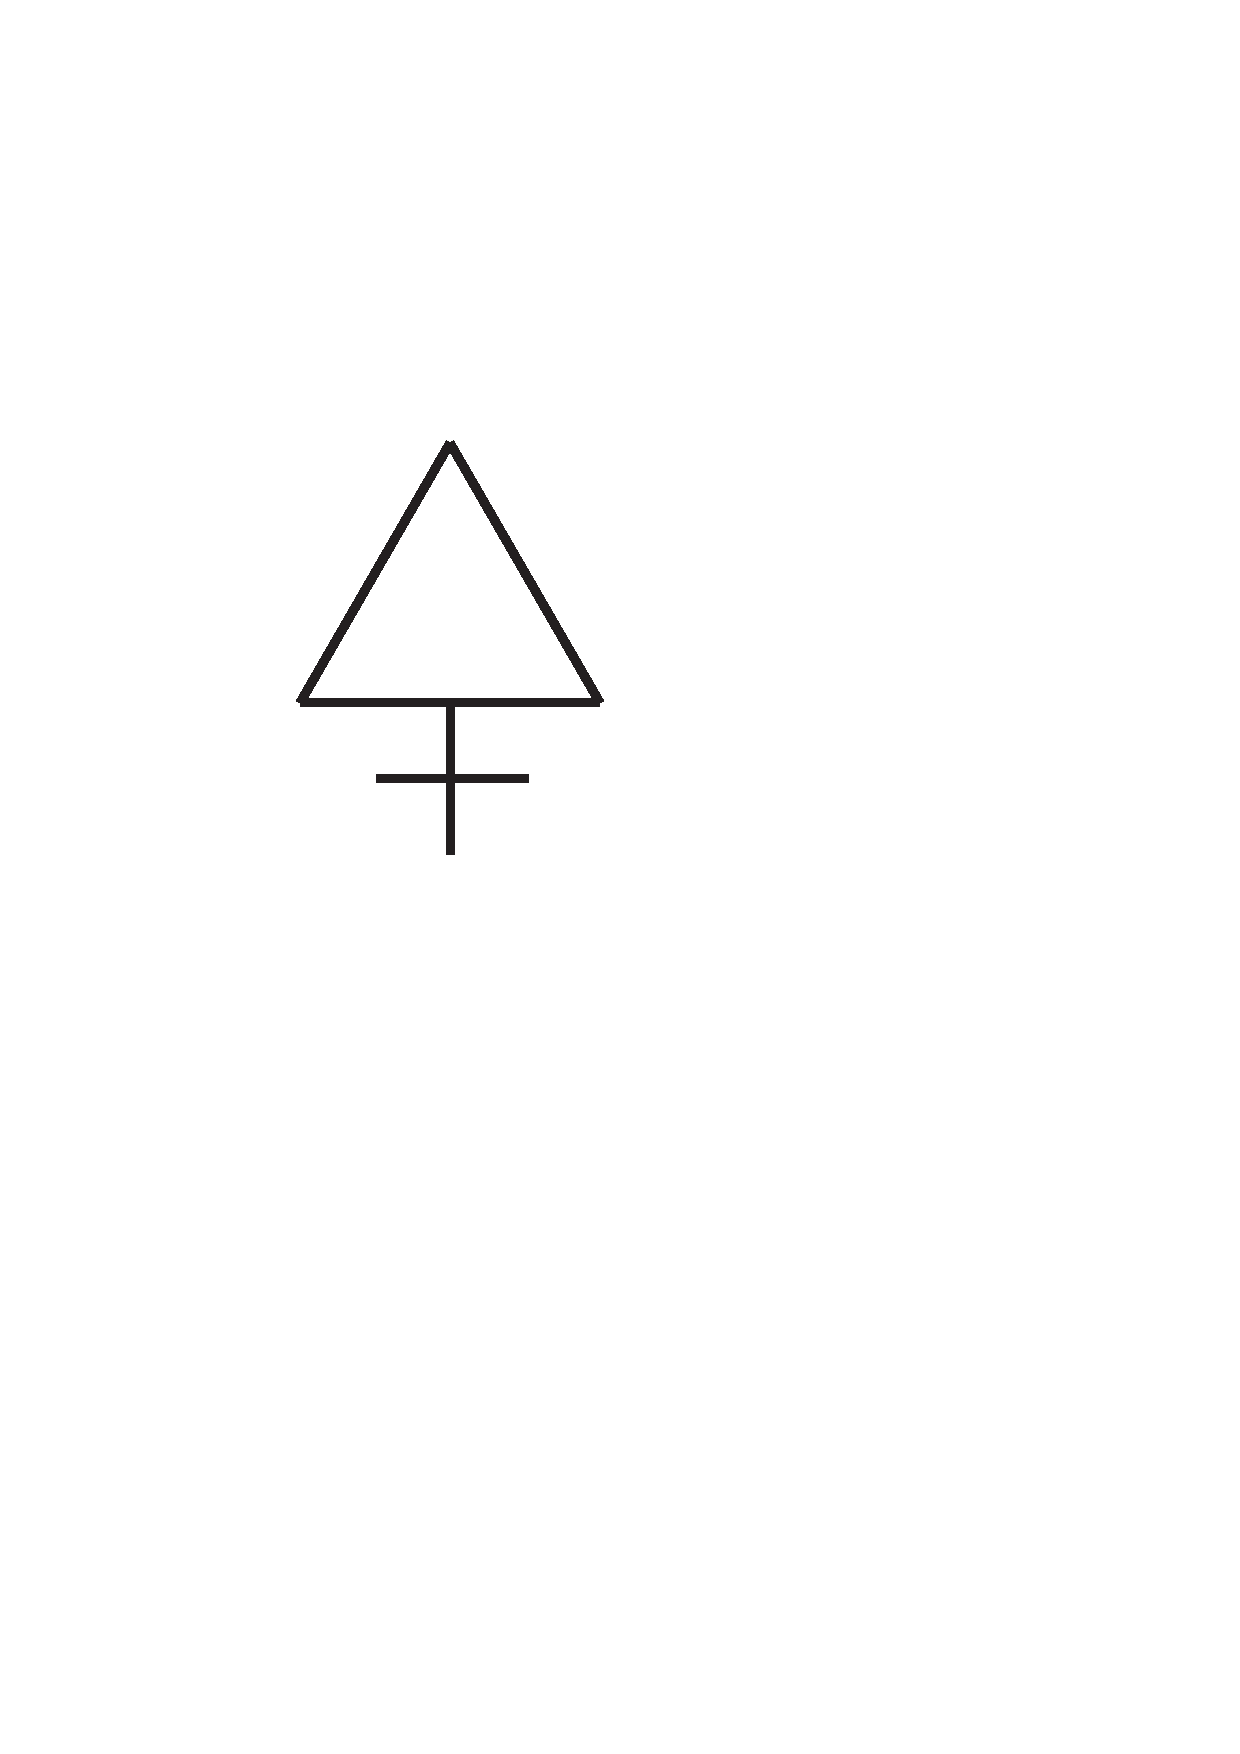
\includegraphics[width=0.02\textwidth]{images/sym-sulph.pdf} & Schwefel\\
$\rightmoon$ & Silber (Mond)\\
% \protect
\includegraphics[width=0.02\textwidth]{images/taros.pdf} & Tartar\\
\protect
\includegraphics[width=0.02\textwidth]{images/vitriol.pdf} & Vitriol\\
$\bigtriangleup$ & Wasser\\
\protect
\includegraphics[width=0.02\textwidth]{images/sym-spirvini.pdf} & Weingeist (Spiritus vini)\\
\protect
\includegraphics[width=0.02\textwidth]{images/taros.pdf} & Weinstein (Tartar)\\
\jupiter & Zinn (Jupiter)
\end{longtable}
\vspace{2.0ex}
%%%%
%%%%
\newpage

\noindent\footnotesize{\uppercase{5. Mathematische Zeichen}}
\setlength\LTleft{0pt} \setlength\LTright{0pt}
\begin{longtable}{lp{100mm}}
\footnotesize\vspace*{1mm}
$\smallfrown$ & Multiplikation\\\vspace*{1mm}
$\smallsmile$ & Division\\\vspace*{1mm}
$\bigtriangledown$ & Dreieck\\\vspace*{1mm}
\rule{1pt}{3mm} & K\"{u}rzung eines Bruchs\\\vspace*{1mm}
$f$ & facit\\\vspace*{1mm}
$\square$ \fbox{2} & Quadrat\\\vspace*{1mm}
\fbox{3}~~cub. & Kubus\\\vspace*{1mm}
$\surd~~~\sqrt{~~~}$\ \ Rq. & Quadratwurzel\\\vspace*{1mm}
=\ aequ.\ aeq.\ $\sqcap$ $\rightpropto$ & gleich\\
$\groesser$ & gr\"{o}{\ss}er als\\
$\kleiner$ & kleiner als\\ \vspace*{1mm}
$\infty$ & unendlich\\
, ,, ,,, $\llcorner \lrcorner$ & Klammerausdr\"{u}cke\\\vspace*{1mm}
\ovalbox{\makebox[15mm][l]{~~~}} & Umrahmungen zur Bezeichnung wegfallender Terme\\\vspace*{1mm}
... & Platzhalter f\"{u}r Terme\\
$\pPsMs$\ $\pleibdashv$ & kombinierte Vorzeichen% $+-$
\\
$\pMsPs$\ $\pleibvdash$% & kombinierte Vorzeichen $-+$
\\
$\pPsPsMs$\ $\ppmE$\ $\ppmG$% & kombinierte Vorzeichen $+(+-)$
\\
$\pPsMsPs$\ $\ppmH$% & kombinierte Vorzeichen $+(-+)$
\\
$\pMsPsMs$%\ & kombinierte Vorzeichen ??$-(+-)$ % oder: plus minus plus ??
\\
$\pMsMsPs$%\ & kombinierte Vorzeichen ??$-(-+)$ % oder: minus plus plus ??
\\
$\pMsPsPs$\ $\ppmD$% & kombinierte Vorzeichen $-(++)$
\end{longtable}
\vspace{2.0ex}
%%%%
%%%%

\noindent\footnotesize{\uppercase{6. Zeichen von Masseinheiten}}
\setlength\LTleft{0pt} \setlength\LTright{0pt}
\begin{longtable}{lp{100mm}}
\footnotesize\vspace*{1mm}
\protect
\includegraphics[width=0.011\textwidth]{images/drachma.pdf} & Drachme\\
\protect
\includegraphics[width=0.022\textwidth]{images/semidrachma.pdf} & halbe Drachme\\\vspace*{1mm}
\protect
\includegraphics[width=0.023\textwidth]{images/semiuncia.pdf} & halbe Unze\\
\Pfund & Pfund\\\vspace*{1,2mm}
\protect
\includegraphics[width=0.018\textwidth]{images/sym-scrupulus.pdf} & Skrupel\\
\protect
\includegraphics[width=0.011\textwidth]{images/uncia.pdf} & Unze
\end{longtable}
\vspace{2.0ex}
%%%%
%%%%

\noindent\footnotesize{\uppercase{7. Sonstige Zeichen}}
\setlength\LTleft{0pt} \setlength\LTright{0pt}
\begin{longtable}{lp{100mm}}
\footnotesize
\Denarius & destilletur, distilletur (noch zu bedenken)\\
\textrecipe & recipe (Rezeptur)
\end{longtable}
\vspace{2.0ex}
%%%%
%%%%


 \newpage
% \vspace*{4.0ex}% PR: Rein provisorisch!
% \renewcommand*{\chapter}{\OrigChapter}


% \noindent\normalsize{\uppercase{Sonderzeichen für Herrn Bayuk}}\vspace*{3mm}
% \setlength\LTleft{0pt} \setlength\LTright{0pt}
% \begin{longtable}{lp{100mm}}
% \normalsize\vspace*{3mm}
% $\pmA$\ $\ppmA$ & \textit{Bedeutung:} $-(-+)$ \ \textit{Befehl:} $\backslash$pmA \textit{bzw.} $\backslash$ppmA \textit{(gesenkt)}\\
% $\pmB$\ $\ppmB$ & \textit{Bedeutung:} $-(+-)$ \ \textit{Befehl:} $\backslash$pmB \textit{bzw.} $\backslash$ppmB \textit{(gesenkt)}
% \end{longtable}
% \vspace{2.0ex}
%%%%
%%%%


% ENDE DER VERZEICHNISSE